\section{流密码:使用 PRG 进行加密}\label{sec:3-2}

令 $G$ 是一个定义在 $(\{0,1\}^\ell,\{0,1\}^L)$ 上的 PRG;也就是说,$G$ 将一个 $\ell$ 比特的种子拉伸为一个 $L$ 比特的输出。由 $G$ 构建的\textbf{流密码} $\mathcal E=(E,D)$ 定义在 $(\{0,1\}^\ell,\{0,1\}^{\leq L},\{0,1\}^{\leq L})$ 上;对于 $s\in\{0,1\}^\ell$ 和 $m,c\in\{0,1\}^{\leq L}$,加密和解密定义如下:如果 $|m|=v$,则:
$$
E(s,m)=G(s)[0\dots v-1]\oplus m
$$
如果 $|c| = v$,则:
$$
D(s,c)=G(s)[0\dots v-1]\oplus c
$$
读者很容易验证,上述加解密方案能够满足我们对密码的定义(特别是满足了正确性属性)。

请注意,为了分析 $\mathcal E$ 的语义安全性,在攻击游戏 \ref{game:2-1} 中与信息 $m$ 相关的长度就是$m$的自然比特长度 $|m|$。此外还需注意,如果 $v$ 比 $L$ 小得多,那么对于许多实际的 PRG 来说,计算 $G(s)$ 的前 $v$ 位有可能比计算出 $G(s)$ 的所有位然后截断要快得多。

本节的主要结论如下:

\begin{theorem}\label{theo:3-1}
如果 $G$ 是一个安全的 PRG,那么由 $G$ 构建的流密码 $\mathcal E$ 就是一个语义安全的密码。
\begin{quote}
特别地,对于每个如攻击游戏 \ref{game:2-1} 中那样攻击 $\mathcal E$ 的 SS 对手 $\mathcal A$,都存在一个如攻击游戏 \ref{game:3-1} 中那样攻击 $G$ 的 PRG 对手 $\mathcal B$,其中 $\mathcal B$ 是一个围绕 $\mathcal A$ 的基本包装器,满足:
\end{quote}
\begin{equation}\label{eq:3-2}
{\rm SS\mathsf{adv}}[\mathcal{A},\mathcal{E}]=2\cdot{\rm PRG\mathsf{adv}}[\mathcal{B},G]
\end{equation}
\end{theorem}

\begin{proof}[证明思路]
基本思想是,我们可以用一个真随机字符串来替换 PRG 的输出,而不会使得对手的优势增长超过一个不可忽略不计的量。然而,在进行这种替换后,对手的优势为零。
\end{proof}

\begin{proof}
令 $\mathcal A$ 是一个如攻击游戏 \ref{game:2-1} 中那样的攻击 $\mathcal E$ 的有效对手。我们想要证明,如果 $G$ 是一个安全的 PRG,那么 ${\rm SS\mathsf{adv}}[\mathcal{A},\mathcal{E}]$ 可以忽略不计。用语义安全攻击游戏的比特猜测版本更为方便。我们证明:
\begin{equation}\label{eq:3-3}
{\rm SS\mathsf{adv}}^∗[\mathcal{A},\mathcal{E}]={\rm PRG\mathsf{adv}}[\mathcal{B},G]
\end{equation}
对于某个有效对手$\mathcal{B}$成立。那么式 \ref{eq:3-2} 就可以由定理 \ref{theo:2-10} 推出。此外,由于我们假设 $G$ 是一个安全的 PRG,那么 ${\rm PRG\mathsf{adv}}[\mathcal{B},G]$ 的值一定是可忽略不计的,因此 ${\rm SS\mathsf{adv}}[\mathcal{A},\mathcal{E}]$ 也是可忽略不计的。

所以,考虑对手 $\mathcal A$ 在攻击游戏 \ref{game:2-1} 的比特猜测版本中对 $\mathcal E$ 的攻击。在这个游戏中,$\mathcal{A}$ 向挑战者提供两个相同长度的消息 $m_0$ 和 $m_1$,然后挑战者选择一个随机密钥 $s$ 和一个随机比特 $b$,并在 $s$ 下对 $m_b$ 进行加密,将得到的密文 $c$ 交给 $\mathcal{A}$;最后,$\mathcal A$ 输出一个比特 $\hat b$。如果 $\hat b=b$,则对手 $\mathcal A$ 赢得游戏。

让我们称这个游戏为\textbf{游戏 $\mathbf{0}$}。 挑战者在这个游戏中的逻辑可以表示如下:

\vspace*{5pt}

\hspace*{5pt} 当收到来自 $\mathcal A$ 的 $m_0,m_1\in\{0,1\}^v$,其中$v\leq L$时:\\
\hspace*{50pt} 计算 $b\overset{\rm R}\leftarrow\{0,1\}$\\
\hspace*{50pt} 计算 $s\overset{\rm R}\leftarrow\{0,1\}^l$,$r\leftarrow G(s)$\\
\hspace*{50pt} 计算 $c\leftarrow r[0\dots v-1]\oplus m_b$\\
\hspace*{50pt} 将 $c$ 发送给 $\mathcal A$。

\vspace*{5pt}

\noindent
图 \ref{fig:3-2} 展示了游戏 $0$ 的流程。

\begin{figure}
  \centering
  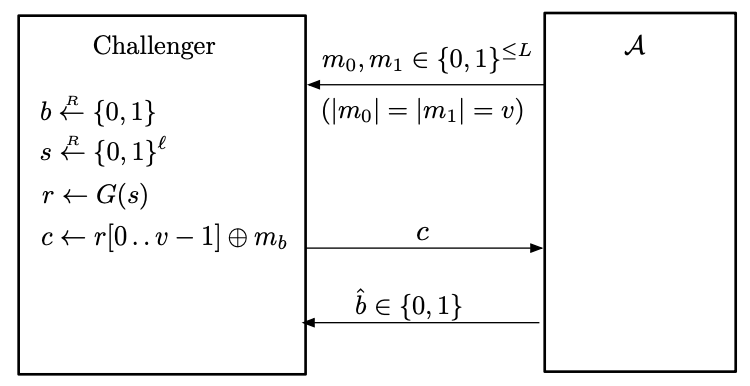
\includegraphics[width=0.5\linewidth]{figures/chapter3/fig2.png}
  \caption{定理 \ref{theo:3-1} 的证明中的游戏 $0$}
  \label{fig:3-2}
\end{figure}

记 $W_0$ 为游戏 $0$ 中 $\hat b=b$ 的事件。根据定义,我们有:
\begin{equation}\label{eq:3-4}
{\rm SS\mathsf{adv}}^∗[\mathcal{A},\mathcal{E}]=|\Pr[W_0]-{1}/{2}|
\end{equation}

接下来,我们修改游戏 $0$ 中挑战者的逻辑,得到一个新的游戏,我们称之为\textbf{游戏 $\mathbf{1}$}。游戏 $1$ 与游戏 $0$基本相同,只是挑战者现在会用一个真随机字符串代替伪随机字符串。游戏 $1$ 中挑战者的逻辑如下:

\vspace*{5pt}

\hspace*{5pt} 当收到来自 $\mathcal A$ 的 $m_0,m_1\in\{0,1\}^v$,其中$v\leq L$时:\\
\hspace*{50pt} 计算 $b\overset{\rm R}\leftarrow\{0,1\}$\\
\hspace*{47pt} \colorbox{gray!50}{计算 $r\overset{\rm R}\leftarrow\{0,1\}^L$}\\
\hspace*{50pt} 计算 $c\leftarrow r[0\dots v-1]\oplus m_b$\\
\hspace*{50pt} 将 $c$ 发送给 $\mathcal A$。

\vspace*{5pt}

与之前一样,$\mathcal A$ 在该游戏结束时输出一个比特 $\hat b$。我们用灰色强调了和游戏$0$之间的差别。图 \ref{fig:3-3} 展示了游戏$1$的流程。

\begin{figure}
  \centering
  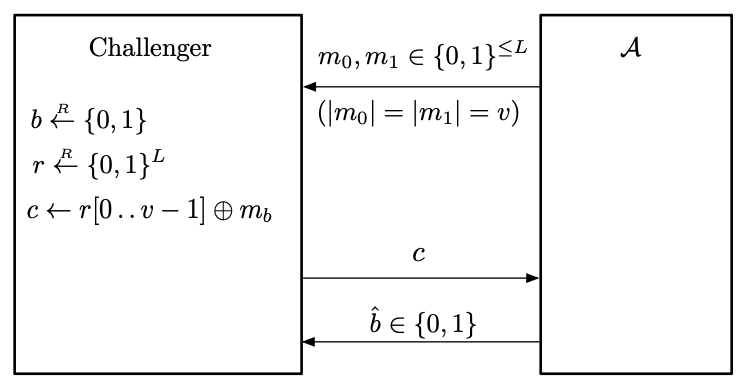
\includegraphics[width=0.5\linewidth]{figures/chapter3/fig3.png}
  \caption{定理 \ref{theo:3-1} 的证明中的游戏 $1$}
  \label{fig:3-3}
\end{figure}

记 $W_1$ 为游戏 $1$ 中 $\hat b=b$ 的事件。我们声称:
\begin{equation}\label{eq:3-5}
\Pr[W_1]={1}/{2}
\end{equation}
这是因为在游戏 $1$ 中,对手事实上攻击的是变长一次性密码本。特别地,很容易看到,对手的输出 $\hat b$ 和挑战者的隐藏比特 $b$ 是相互独立的。

最后,我们展示如何构建一个有效 PRG 对手 $\mathcal B$,它将 $\mathcal A$ 作为一个子程序,使得:
\begin{equation}\label{eq:3-6}
|\Pr[W_0]-\Pr[W_1]|={\rm PRG\mathsf{adv}}[\mathcal{B},G]
\end{equation}
成立。这实际上非常简单。我们的新对手 $\mathcal B$ 的逻辑如图 \ref{fig:3-4} 所示。这里,$\delta$的定义如下:
\begin{equation}\label{eq:3-7}
\delta(x,y)=
\left\{
\begin{array}{ll}
1, & x=y\\
0, & x\neq y
\end{array}
\right.
\end{equation}
另外,标有``PRG 挑战者"的方框扮演攻击游戏 \ref{game:3-1} 中 $G$ 的挑战者的角色。

\begin{figure}
  \centering
  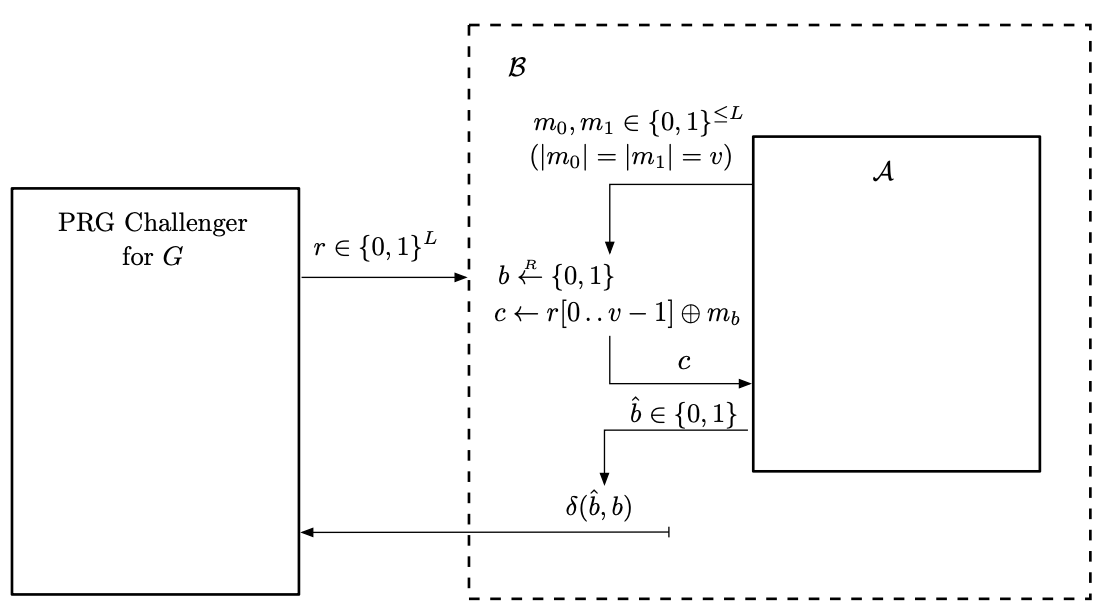
\includegraphics[width=0.75\linewidth]{figures/chapter3/fig4.png}
  \caption{定理 \ref{theo:3-1} 的证明中的PRG对手$\mathcal{B}$}
  \label{fig:3-4}
\end{figure}

换句话说,对手 $\mathcal B$ 是一个(如攻击游戏 \ref{game:3-1} 中那样)旨在攻击 $G$ 的 PRG 对手,它从它的 PRG 挑战者那里收到 $r\in\{0,1\}^L$,然后扮演 $\mathcal A$ 的挑战者角色,如下所示:

\vspace*{5pt}

\hspace*{5pt} 当收到来自 $\mathcal A$ 的 $m_0,m_1\in\{0,1\}^v$,其中$v\leq L$时:\\
\hspace*{50pt} 计算 $b\overset{\rm R}\leftarrow\{0,1\}$\\
\hspace*{50pt} 计算 $c\leftarrow r[0\dots v-1]\oplus m_b$\\
\hspace*{50pt} 将 $c$ 发送给 $\mathcal A$。

\vspace*{5pt}

\noindent
最后,当 $\mathcal A$ 输出一个比特 $\hat b$ 时,$\mathcal B$ 输出比特 $\delta(\hat b,b)$。

令 $p_0$ 为 PRG 挑战者在运行攻击游戏 \ref{game:3-1} 的实验 $0$ 时,$\mathcal B$ 输出 $1$ 的概率,令 $p_1$ 为 PRG 挑战者运行攻击游戏 \ref{game:3-1} 的实验 $1$ 时,对手 $\mathcal B$ 输出 $1$ 的概率。根据定义,${\rm PRG\mathsf{adv}}[\mathcal{A},G]=|p_1-p_0|$。此外,如果 PRG 挑战者正在运行实验 $0$,那么对手 $\mathcal A$ 本质上就是在进行我们这里的游戏 $0$,所以有 $p_0=\Pr[W_0]$;而如果 PRG 挑战者正在进行实验  $1$,那么对手 $\mathcal A$ 本质上就是在进行我们这里的游戏 $1$,所以有$p_1=\Pr[W_1]$。于是我们立即就能得到式 \ref{eq:3-6}。

结合式 \ref{eq:3-4},\ref{eq:3-5} 和 \ref{eq:3-6},我们就可得到式\ref{eq:3-3}。
\end{proof}

在上述定理中,我们将 $\mathcal E$ 的安全性归约到 $G$ 的安全性上,并表明如果 $\mathcal A$ 是一个攻击 $\mathcal E$ 的有效语义安全对手,那么存在一个攻击 $G$ 的有效 PRG 对手 $\mathcal B$,使得:
$$
{\rm SS\mathsf{adv}}[\mathcal{A},\mathcal{E}]\leq 2\cdot{\rm PRG\mathsf{adv}}[\mathcal{B},G]
$$
(实际上,我们还证明了等号是成立的,但这并不重要。)在证明中,我们认为如果 $G$ 是安全的,那么 ${\rm PRG\mathsf{adv}}[\mathcal{B},G]$ 的值可忽略不计。因此,根据上述不等式,我们得出结论,${\rm SS\mathsf{adv}}[\mathcal{A},\mathcal{E}]$ 也是可忽略不计的。由于这对所有的有效对手 $\mathcal A$ 都成立,于是我们可以得出结论,$\mathcal E$ 是语义安全的。

类似于定理 \ref{theo:2-7} 之后的讨论,另一种结构化的证明方法是反证法:事实上,如果我们假设 $\mathcal E$ 是不安全的,那么一定有一个有效对手 $\mathcal A$ 能使得 ${\rm SS\mathsf{adv}}[\mathcal{A},\mathcal{E}]$ 的值不可忽略不计。而安全归约(以及上述不等式)赋予我们一个有效对手 $\mathcal B$,使得 ${\rm PRG\mathsf{adv}}[\mathcal{B},G]$ 的值也不可忽略不计。也就是说,如果我们能破解 $\mathcal E$,我们也就能破解 $G$。虽然这在逻辑上是等价的,但这样的证明有一种不同的``感觉":我们从破解 $\mathcal E$ 的对手 $\mathcal A$ 开始,并说明如何使用 $\mathcal A$ 来构造一个能破解 $G$ 的新对手 $\mathcal B$。

读者应该注意到,上述定理的证明与我们在 \ref{subsec:2-2-4} 小节中对网络电子轮盘赌的分析遵循基本相同的模式。在这两种情况下,我们都从一个攻击游戏开始(图 \ref{fig:2-2} 和图 \ref{fig:3-2}),我们对其进行修改,从而得到一个新的攻击游戏(图 \ref{fig:2-3} 和图 \ref{fig:3-3});而在这个新的攻击游戏中,计算对手的优势非常容易。此外,我们还使用了一个适当的安全假设,以证明对手在原始游戏和修改后的游戏中的优势差异是可忽略不计的。这是通过引入一个新的对手(图 \ref{fig:2-4} 和图 \ref{fig:3-4})来实现的,该对手攻击底层的密码学原语(密码或 PRG),其优势等于这一差异。假设底层原语是安全的,那么这个差异一定是可忽略不计的;或者,我们可以反过来说:如果这个差异是不可忽略不计的,那么新对手就会``破坏"底层密码学原语。

这是一个将在本文中反复出现的模式。因此读者应该仔细研究这种两种分析方法,以确保能够完全理解其中的原理。